\hypertarget{crapahutages-sur-la-moscova}{%
\section{Crapahutages sur la
Moscova}\label{crapahutages-sur-la-moscova}}

\emph{Dimanche 03 juin 2018}

Nous venons de passer 6 jours à Moscou, que nous avons exploré en long,
en large, en travers, mais surtout à pied ! La marche y est très
agréable : les trottoirs sont très larges, propres, les bâtiments sont
beaux avec des bas-reliefs et des statues à tout va, et la ville est
globalement plate ce qui facilite grandement les choses :)

Comme ça risque d'être un peu long de raconter tout ce qu'on a vu et
visité, je vais plutôt vous raconter mes impressions et constats sur la
vie à Moscou. Aucune prétention de sociologie, juste des ressentis :

\begin{itemize}
\tightlist
\item
  Moscou c'est grand, pas seulement par la taille de la ville mais par
  la taille de chaque bâtiment, que ce soit la Lubjanka, le parlement,
  la bibliothèque nationale ou des immeubles de HLM, tout est démesuré.
\item
  Moscou c'est joli. Alors je pense qu'il y a un gros biais avec la
  préparation de la coupe du Monde de football qui commence dans quinze
  jours, mais on trouve partout des rues avec un toit de loupiotes, des
  arbres illuminés la nuit dans les parcs, des arcades de fleurs...
\end{itemize}

\begin{figure}
\centering
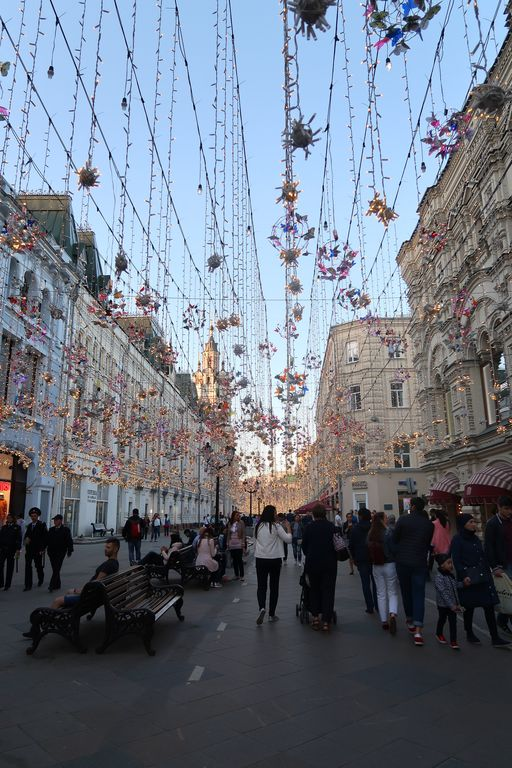
\includegraphics{images/20180603_moscou.JPG}
\caption{La rue Nikolskaya et son plafond de lumière.}
\end{figure}

\begin{itemize}
\tightlist
\item
  à propos de fleurs, si queulqu'un veut faire fortune à Moscou, ça ne
  sert à rien de se lancer dans la pétro-chimie ou dans le caviar, il
  faut faire fleuriste. Ces gens ont un truc avec les fleurs... on
  pourrait dire qu'on vit ici un bouquet à la main.
\item
  le métro est incroyable, surtout pour de bons parisiens que nous
  sommes : c'est grand, c'est propre, ça sent bon (!), et c'est surtout
  un musée à part entière, avec des stations majestueusement décorées et
  toutes différentes les unes des autres. C'est aussi très profond (les
  escalators sont vertigineux) et très bien organisé. J'imagine la tête
  des touristes moscovites à Paris quand ils prennent notre métro pour
  la première fois...
\end{itemize}

\begin{figure}
\centering
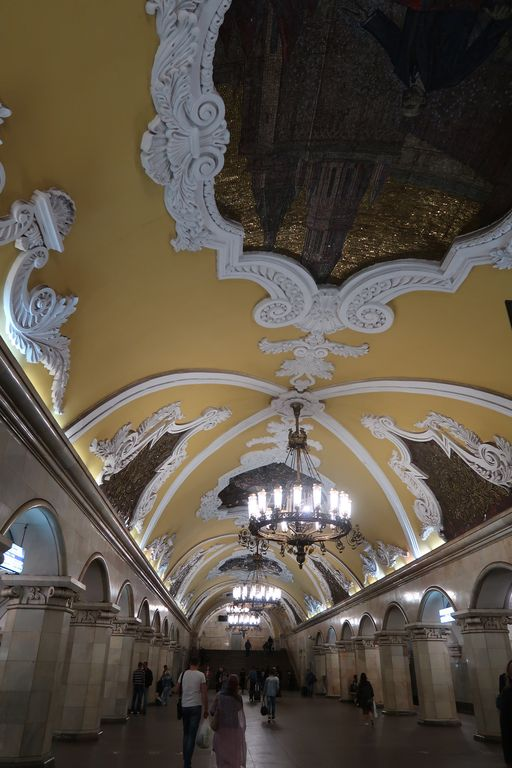
\includegraphics{images/20180603_metro.JPG}
\caption{Les stations de métro sont quasiment des oeuvres d'art !}
\end{figure}

\begin{itemize}
\tightlist
\item
  les femmes moscovites ont du style, vraiment, lookées de la tête aux
  pieds
\item
  par contre, par rapport à nos standards (encore une fois), nous
  n'avons pas trouvé les russes très polis. On ne nous a jamais, ne
  serait-ce qu'une fois, tenu la porte, les gens de l'hôtel ne m'ont
  jamais répondu quand je leur disais bonjour ni au-revoir, on se fait
  souvent bousculer (et je ne parle pas des hordes de touristes en
  groupe, c'est une autre histoire !) et on ne nous a jamais souri à une
  caisse de restaurant ou de supermarché. Heureusement qu'il y a des
  exceptions. Je pense à cette dame qui passait par là et qui, devant
  nos airs paumés nous a spontanément proposé son aide pour retrouver
  notre chemin vers la gare de Léningrad :)
\item
  et l'alphabet cyrillique, on en parle ? Un alphabet avec globalement
  des lettres qu'on connaît, mais t'as une chance sur deux pour que ça
  se prononce pas du tout comme tu crois. Donc, petit cours rapide : le
  P se prononce R, le C se prononce S, le H se prononce N, le Y se
  prononce OU, le grand B se prononce V, le petit b est en fait un grand
  B et se prononce B. Voilà, vous avez tout suivi ? Du coup, si je vous
  écris PECTOPAH, vous le prononcez...? Restaurant ! Bravo, vous êtes
  niveau 1 en cyrillique \textbackslash{}o/. Heureusement que Flo s'en
  sort bien en Russe sinon je serais perdue \^{}\^{}
\item
  dans un autre domaine, la scène musicale est super riche et très
  intéressante. Il y a des concerts de rue à tous les coins,
  généralement de bonne qualité, où les gens s'arrêtent volontiers pour
  écouter, et ça fait une super ambiance
\item
  bon, je crois qu'on parlera pas de la nourriture, les souvenirs du
  Liban sont trop frais encore, on n'est pas prêts ;)
\end{itemize}

D'ailleurs, parce que j'aime bien me contredire, une petite anecdote sur
le gentillesse des russes, qui s'exacerbe avec le nombre de verres
d'alcool absorbés... Un soir, nous rejoignons Irma qui nous promène dans
le quartier de Prospekt Mira (avenue du Monde) jusqu'à une petite place
où elle nous promet de déguster des Cheburieki, spécialité populaire qui
se mange au bar, avec les mains. On arrive impatients (et un peu affamés
aussi) devant le bar en question, qui se trouve être fermé depuis 10
minutes ! Plusieurs groupes de gens en sortent, Irma exerce ses talents
de comédienne en insistant sur les \emph{kilomètres} qu'on a fait pour
arriver là, pour \emph{ces} Cheburieki et qu'elle a amenée des
\emph{invités}... Sous les cris d'Irma, grande comédienne, coup de
théâtre ! L'un des derniers clients sort de l'endroit et nous tend une
assiette de Cheburieki avec un verre de cognac. Il explique que c'est
son anniversaire, et qu'il nous donne tout ça. Quelques secondes plus
tard, le propriétaire de la gargote nous apporte encore un autre
Cheburieke, qu'il nous offre aussi. Nous voilà donc avec trois
Cheburieki qu'on dégute sur la place, tout contents :)

\begin{figure}
\centering
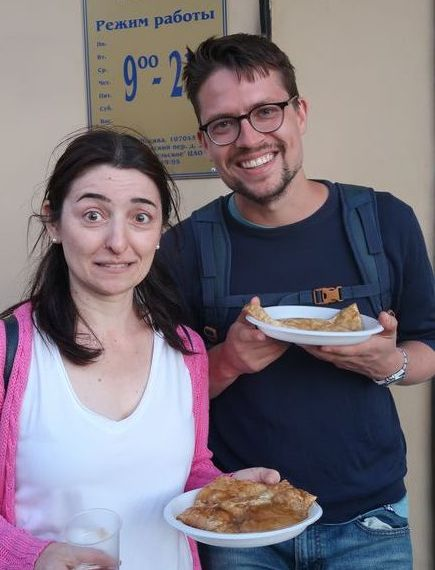
\includegraphics{images/20180603_cheburieki.JPG}
\caption{Les fameux Cheburieki, obtenus grâce à Irma.}
\end{figure}

On vous laisse avec quelques photos (dont l'une a été réalisée avec un
trucage optique, on attend vos commentaires pour savoir si ça se voit).
Prochaine étape : Saint Pétersbourg, la Venise du nord, et ses nuits
blanches.

Et petit bonus réalisé avec la caméra 360° (merci Vaness ;) ).

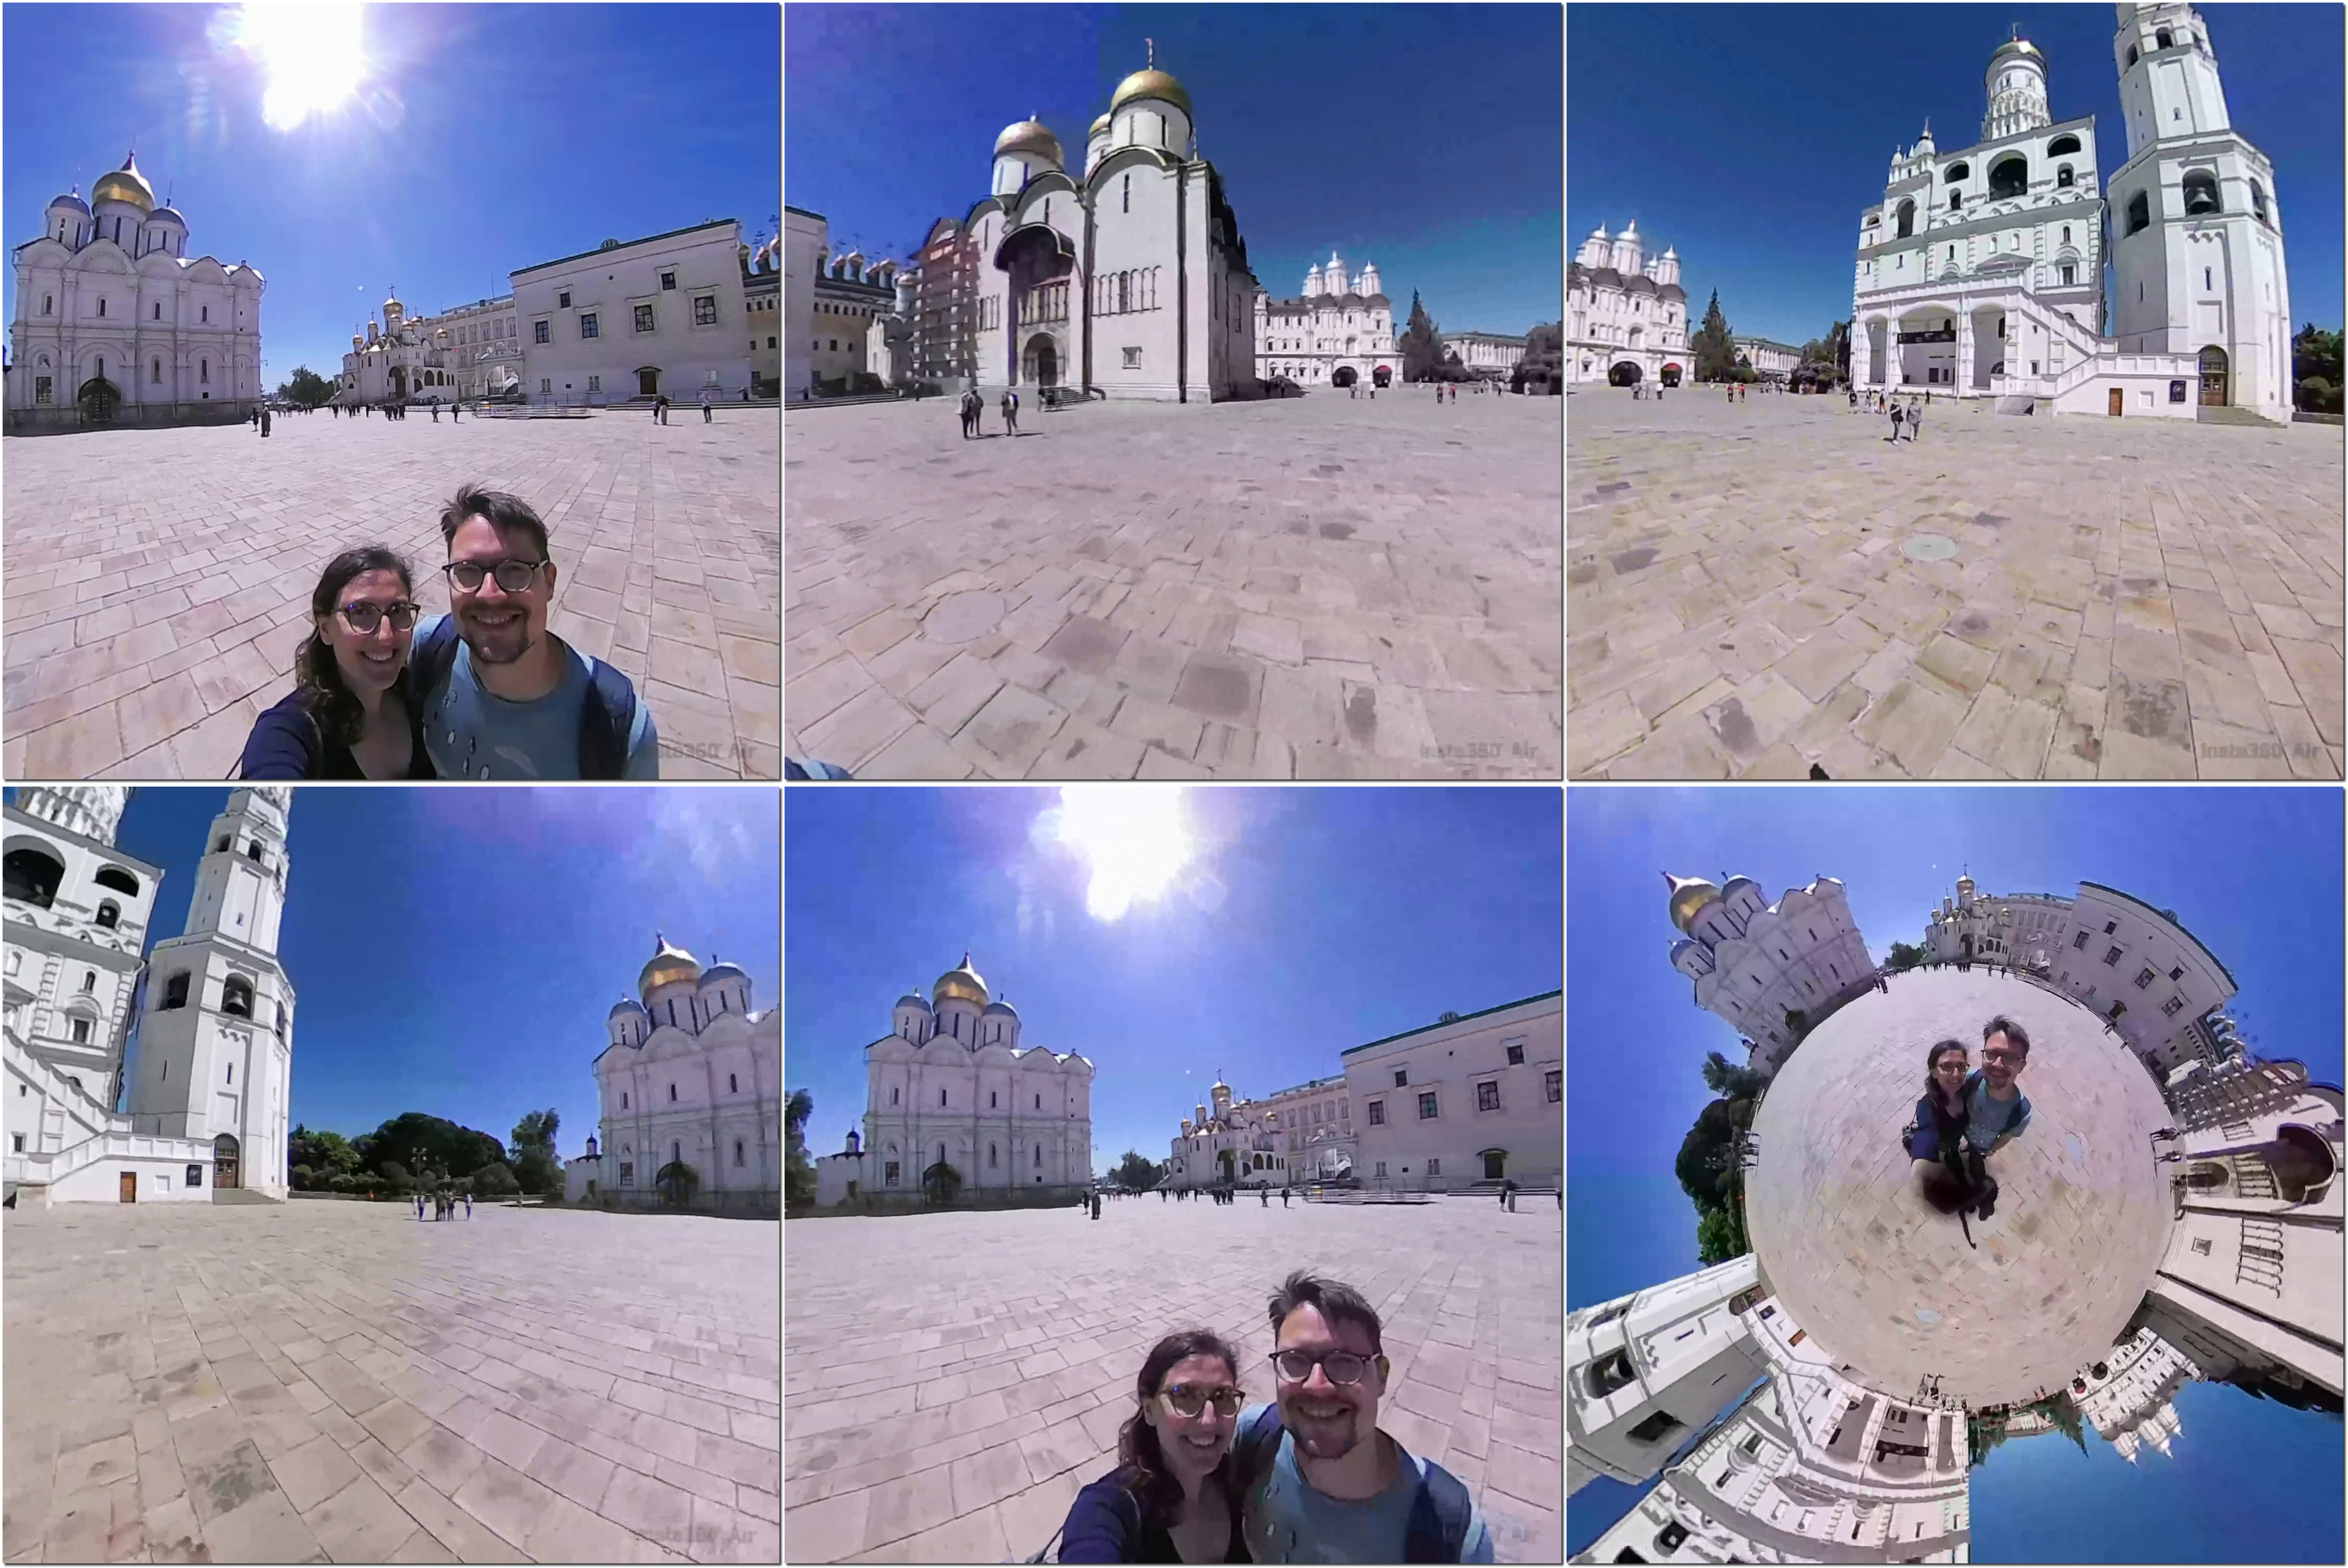
\includegraphics{montage/russie.jpg}

\emph{Elida et Florian}

\hypertarget{commentaires}{%
\subsection{Commentaires}\label{commentaires}}

\begin{itemize}
\item
  ZRC, \emph{2018-06-03 15h48}

  Moi je dis que la statue de la photo 23 ne repose pas exactement sur
  l'eau... Flo aurait pu citer un texte qu'on a vu en cours de russe,
  qui disait que la vie était dure et qu'on ne souriait pas pour rien en
  Russie.
\item
  Thibaud, \emph{2018-06-03 17h59}

  C'est vrai que la photo 23 est chelou.\\
  J'avais lu à peu près la même chose sur les sourires en Russie : on ne
  sourit pas juste par politesse, ça peut d'ailleurs être considéré
  comme offensant !
\item
  Florian LB, \emph{2018-06-03 21h04}

  Je ne savais pas tout ça. Du coup, je viens de taper la requête dans
  mon moteur de recherche favori et il semble que le sourire russe soit
  un point d'interrogation pour beaucoup de gens. Me voilà rassuré. :-)
\item
  Florian LB, \emph{2018-06-03 20h52}

  Ah zut, je ne m'en souviens pas ! Tu crois que tu peux retrouver le
  texte et le mettre ici ?

  En tout cas bravo, tu as trouvé la photo truquée ! On a utilisé un
  écran de smartphone pour donner un reflet de ciel à l'image.
\item
  Timothée Nicolas, \emph{2018-06-03 21h05}

  C'est magnifique et très intéressant ! On a hâte d'en savoir plus !
\end{itemize}

